\documentclass[aspectratio=169,10pt]{beamer}

\usepackage[T1]{fontenc}
\usepackage{lmodern}
\usepackage{graphicx}
\usepackage{booktabs}
\usepackage{tikz}
\usepackage{xcolor}

\definecolor{Ink}{HTML}{20262B}
\definecolor{Navy}{HTML}{17324D}
\definecolor{Teal}{HTML}{168C88}
\definecolor{Amber}{HTML}{D99022}
\definecolor{Red}{HTML}{C94C4C}
\definecolor{Muted}{HTML}{697279}
\definecolor{Mist}{HTML}{E8EEF2}
\definecolor{Wash}{HTML}{F5F8FA}

\setbeamercolor{normal text}{fg=Ink,bg=white}
\setbeamercolor{frametitle}{fg=Navy,bg=white}
\setbeamerfont{frametitle}{size=\Large,series=\bfseries}
\setbeamertemplate{navigation symbols}{}
\setbeamersize{text margin left=.55cm,text margin right=.55cm}
\setbeamertemplate{frametitle}{%
  \vspace{.18cm}\insertframetitle\par\vspace{-.10cm}%
  \color{Teal}\rule{1.0cm}{1.4pt}\color{Mist}\rule{\dimexpr\textwidth-1.0cm\relax}{1.4pt}}
\setbeamertemplate{footline}{%
  \leavevmode\hbox{\begin{beamercolorbox}[wd=.82\paperwidth,ht=2.6ex,dp=1ex,leftskip=.55cm]{normal text}%
  \color{Muted}\scriptsize FOR2107 resting-state comparison · preliminary · 1 September 2026
  \end{beamercolorbox}\begin{beamercolorbox}[wd=.18\paperwidth,ht=2.6ex,dp=1ex,rightskip=.55cm plus1fil]{normal text}%
  \color{Muted}\scriptsize\insertframenumber/4
  \end{beamercolorbox}}}

\newcommand{\sourceNote}[1]{\vspace{.04cm}{\color{Muted}\tiny #1}}
\newcommand{\paneltitle}[1]{{\color{Navy}\bfseries\small #1}}

\begin{document}

\begin{frame}[plain]
  \vfill
  
\begin{tikzpicture}
    \fill[Teal] (0,0) rectangle (1.1,.10);
    \fill[Navy] (1.25,0) rectangle (5.2,.10);
  \end{tikzpicture}
  \vspace{.30cm}

  {\color{Navy}\fontsize{28}{32}\selectfont\bfseries Visual cross-check of resting-state clustering\par}
  \vspace{.18cm}
  {\color{Muted}\Large FOR2107 compared with Tozzi et al.\par}
  \vspace{.48cm}
  {\color{Ink}\normalsize Same layout, different information content: the paper combines rest and task-derived circuit scores; our panels use the 14 resting-state edges currently available.\par}
  \vfill
  {\color{Muted}\small Preliminary comparison · five- and six-cluster descriptive solutions · 1 September 2026}
\end{frame}

\begin{frame}{Supplementary Figure 2: how convincing is the separation?}
\centering
\begin{columns}[T,onlytextwidth]
  \begin{column}{.325\textwidth}
    \centering\paneltitle{Tozzi et al.}\par\vspace{.08cm}
    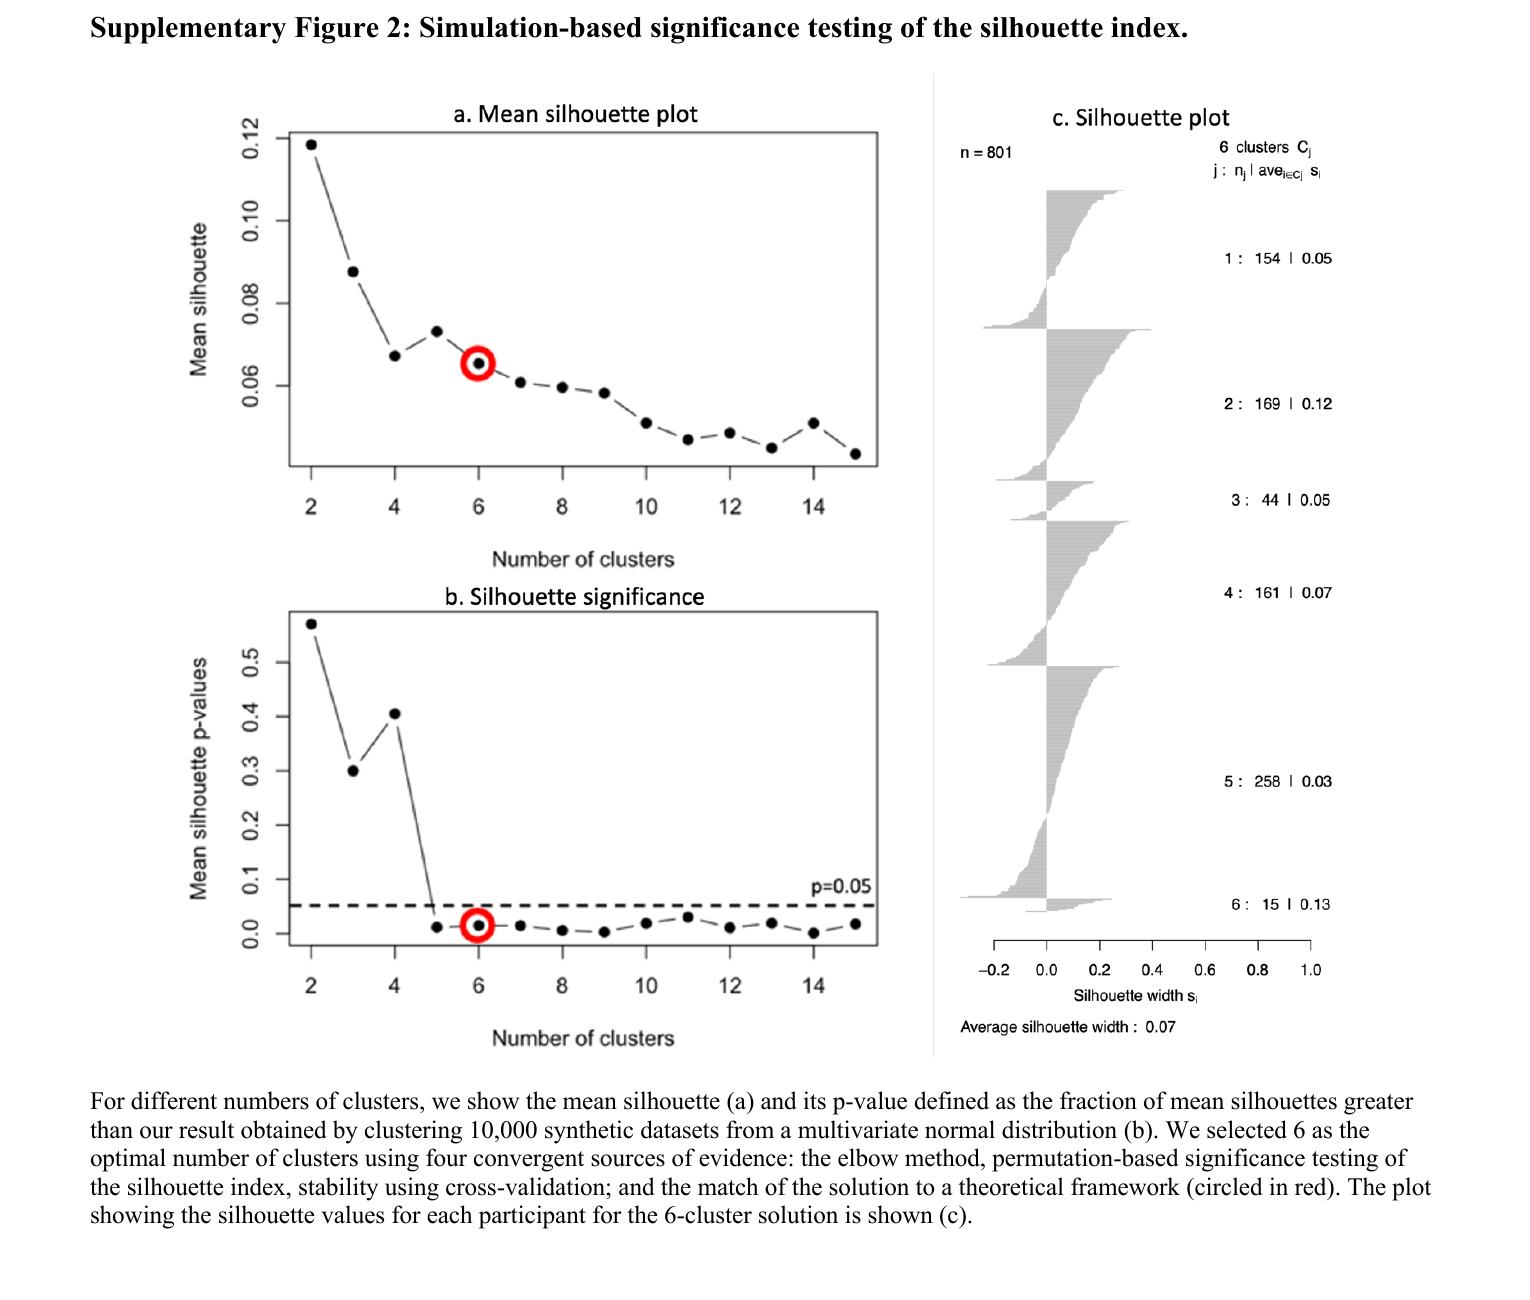
\includegraphics[width=\linewidth,height=.68\textheight,keepaspectratio]{figures/tozzi_supp_fig2.png}\par
  \end{column}
  \begin{column}{.325\textwidth}
    \centering\paneltitle{FOR2107 · k = 6}\par\vspace{.08cm}
    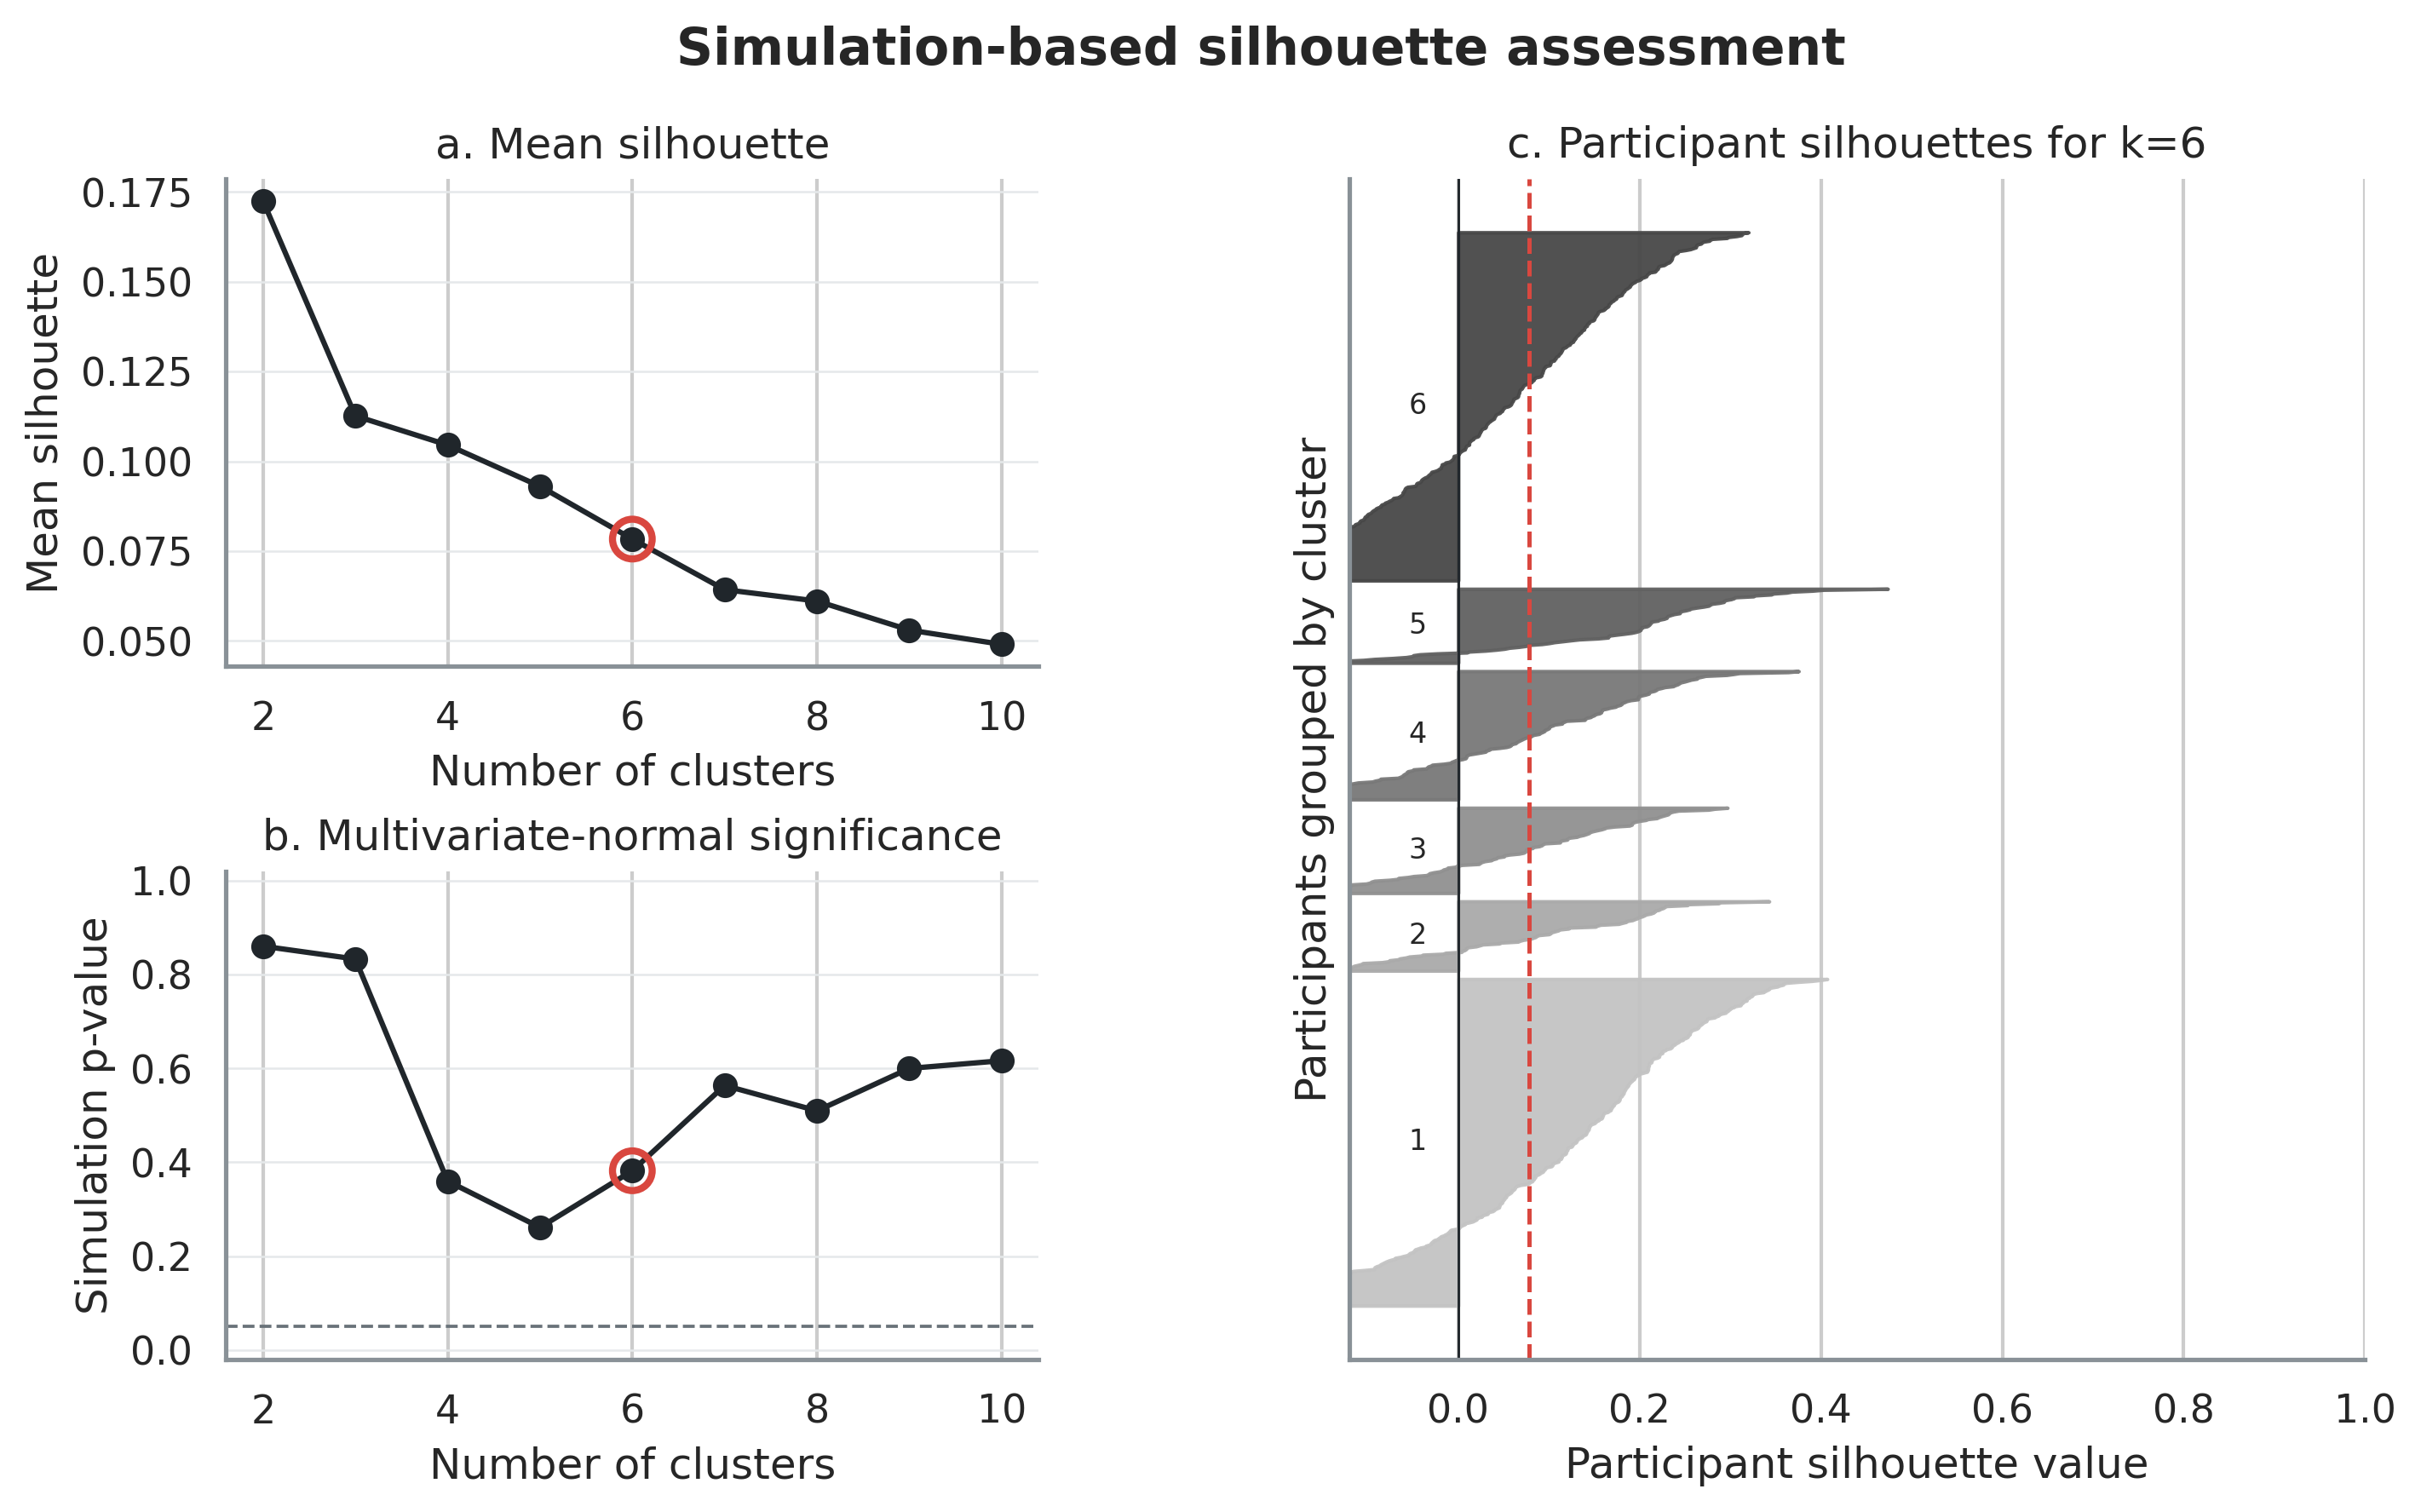
\includegraphics[width=\linewidth,height=.68\textheight,keepaspectratio]{figures/supplementary_figure_2_k6.png}\par
  \end{column}
  \begin{column}{.325\textwidth}
    \centering\paneltitle{FOR2107 · k = 5}\par\vspace{.08cm}
    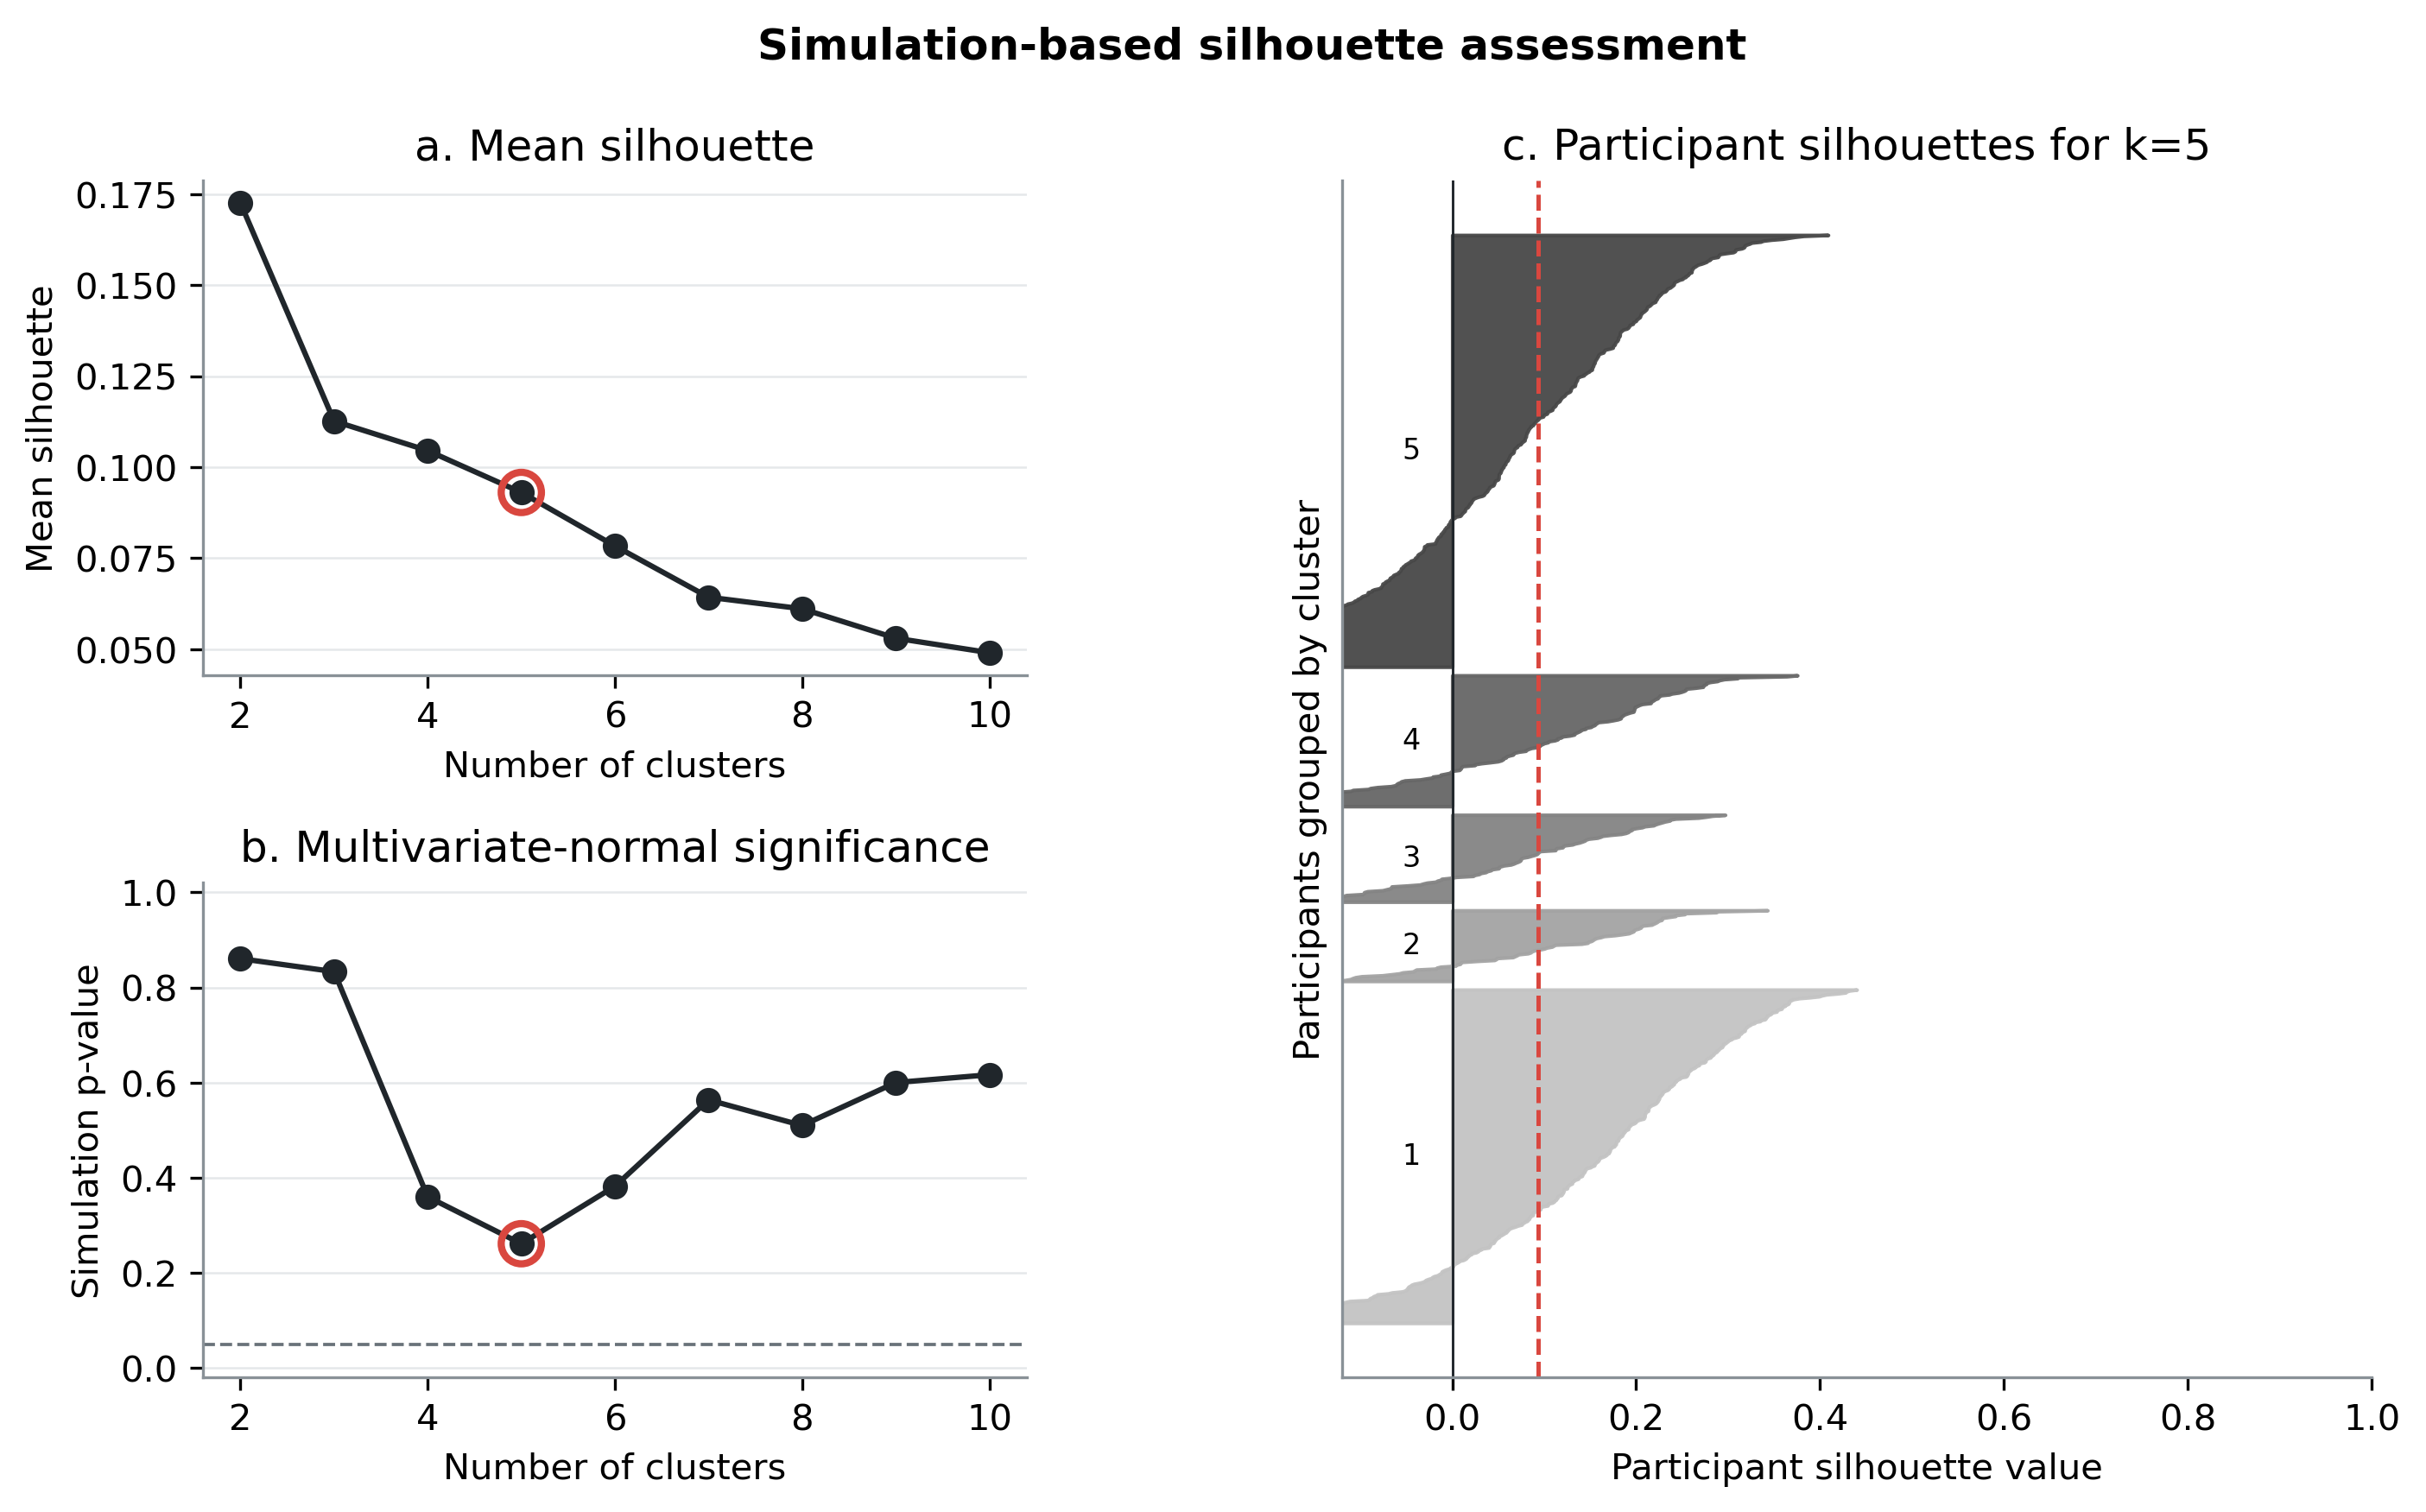
\includegraphics[width=\linewidth,height=.68\textheight,keepaspectratio]{figures/supplementary_figure_2_k5.png}\par
  \end{column}
\end{columns}
\end{frame}

\begin{frame}{Supplementary Figure 5: what do the cluster profiles look like?}
\centering
\begin{columns}[T,onlytextwidth]
  \begin{column}{.325\textwidth}
    \centering\paneltitle{Tozzi et al.}\par\vspace{.06cm}
    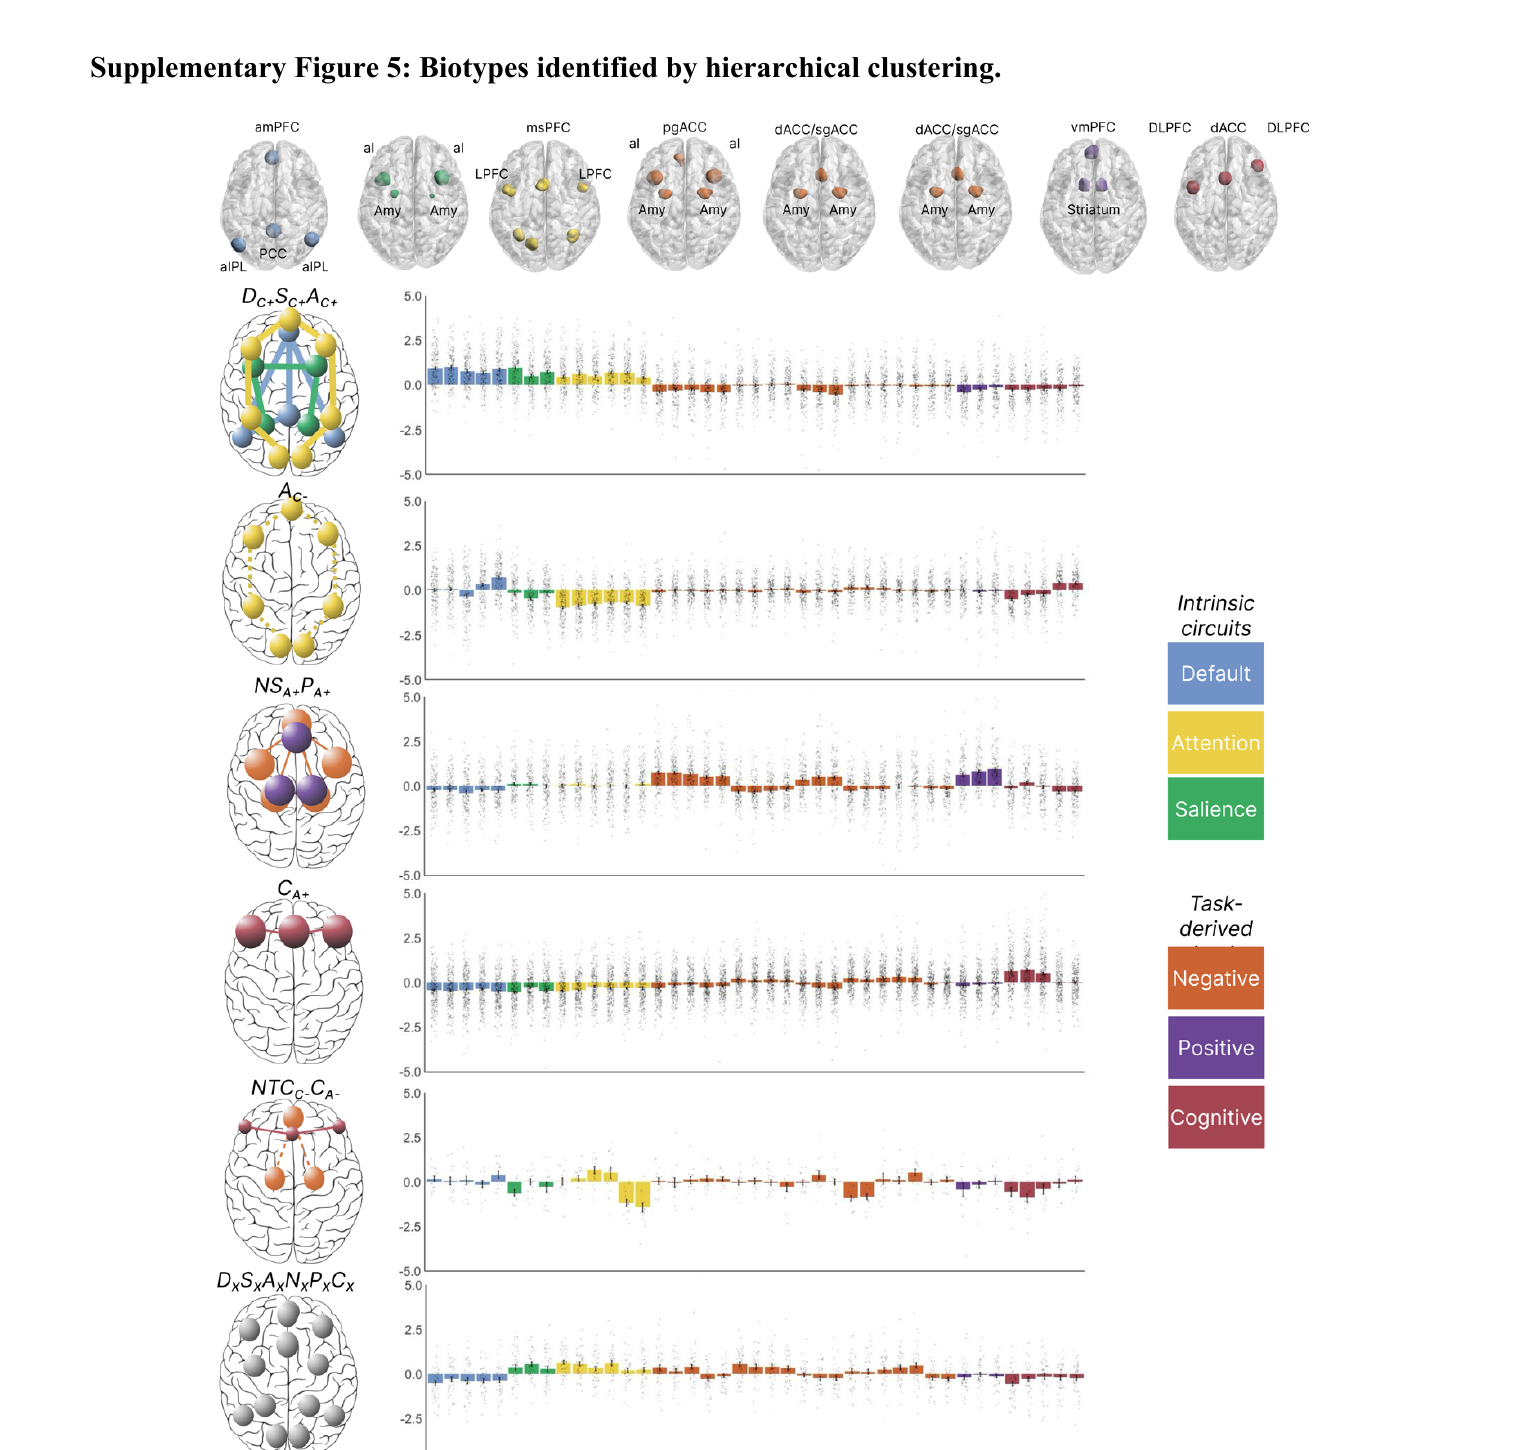
\includegraphics[width=\linewidth,height=.75\textheight,keepaspectratio]{figures/tozzi_supp_fig5.png}\par
  \end{column}
  \begin{column}{.325\textwidth}
    \centering\paneltitle{FOR2107 · k = 6}\par\vspace{.06cm}
    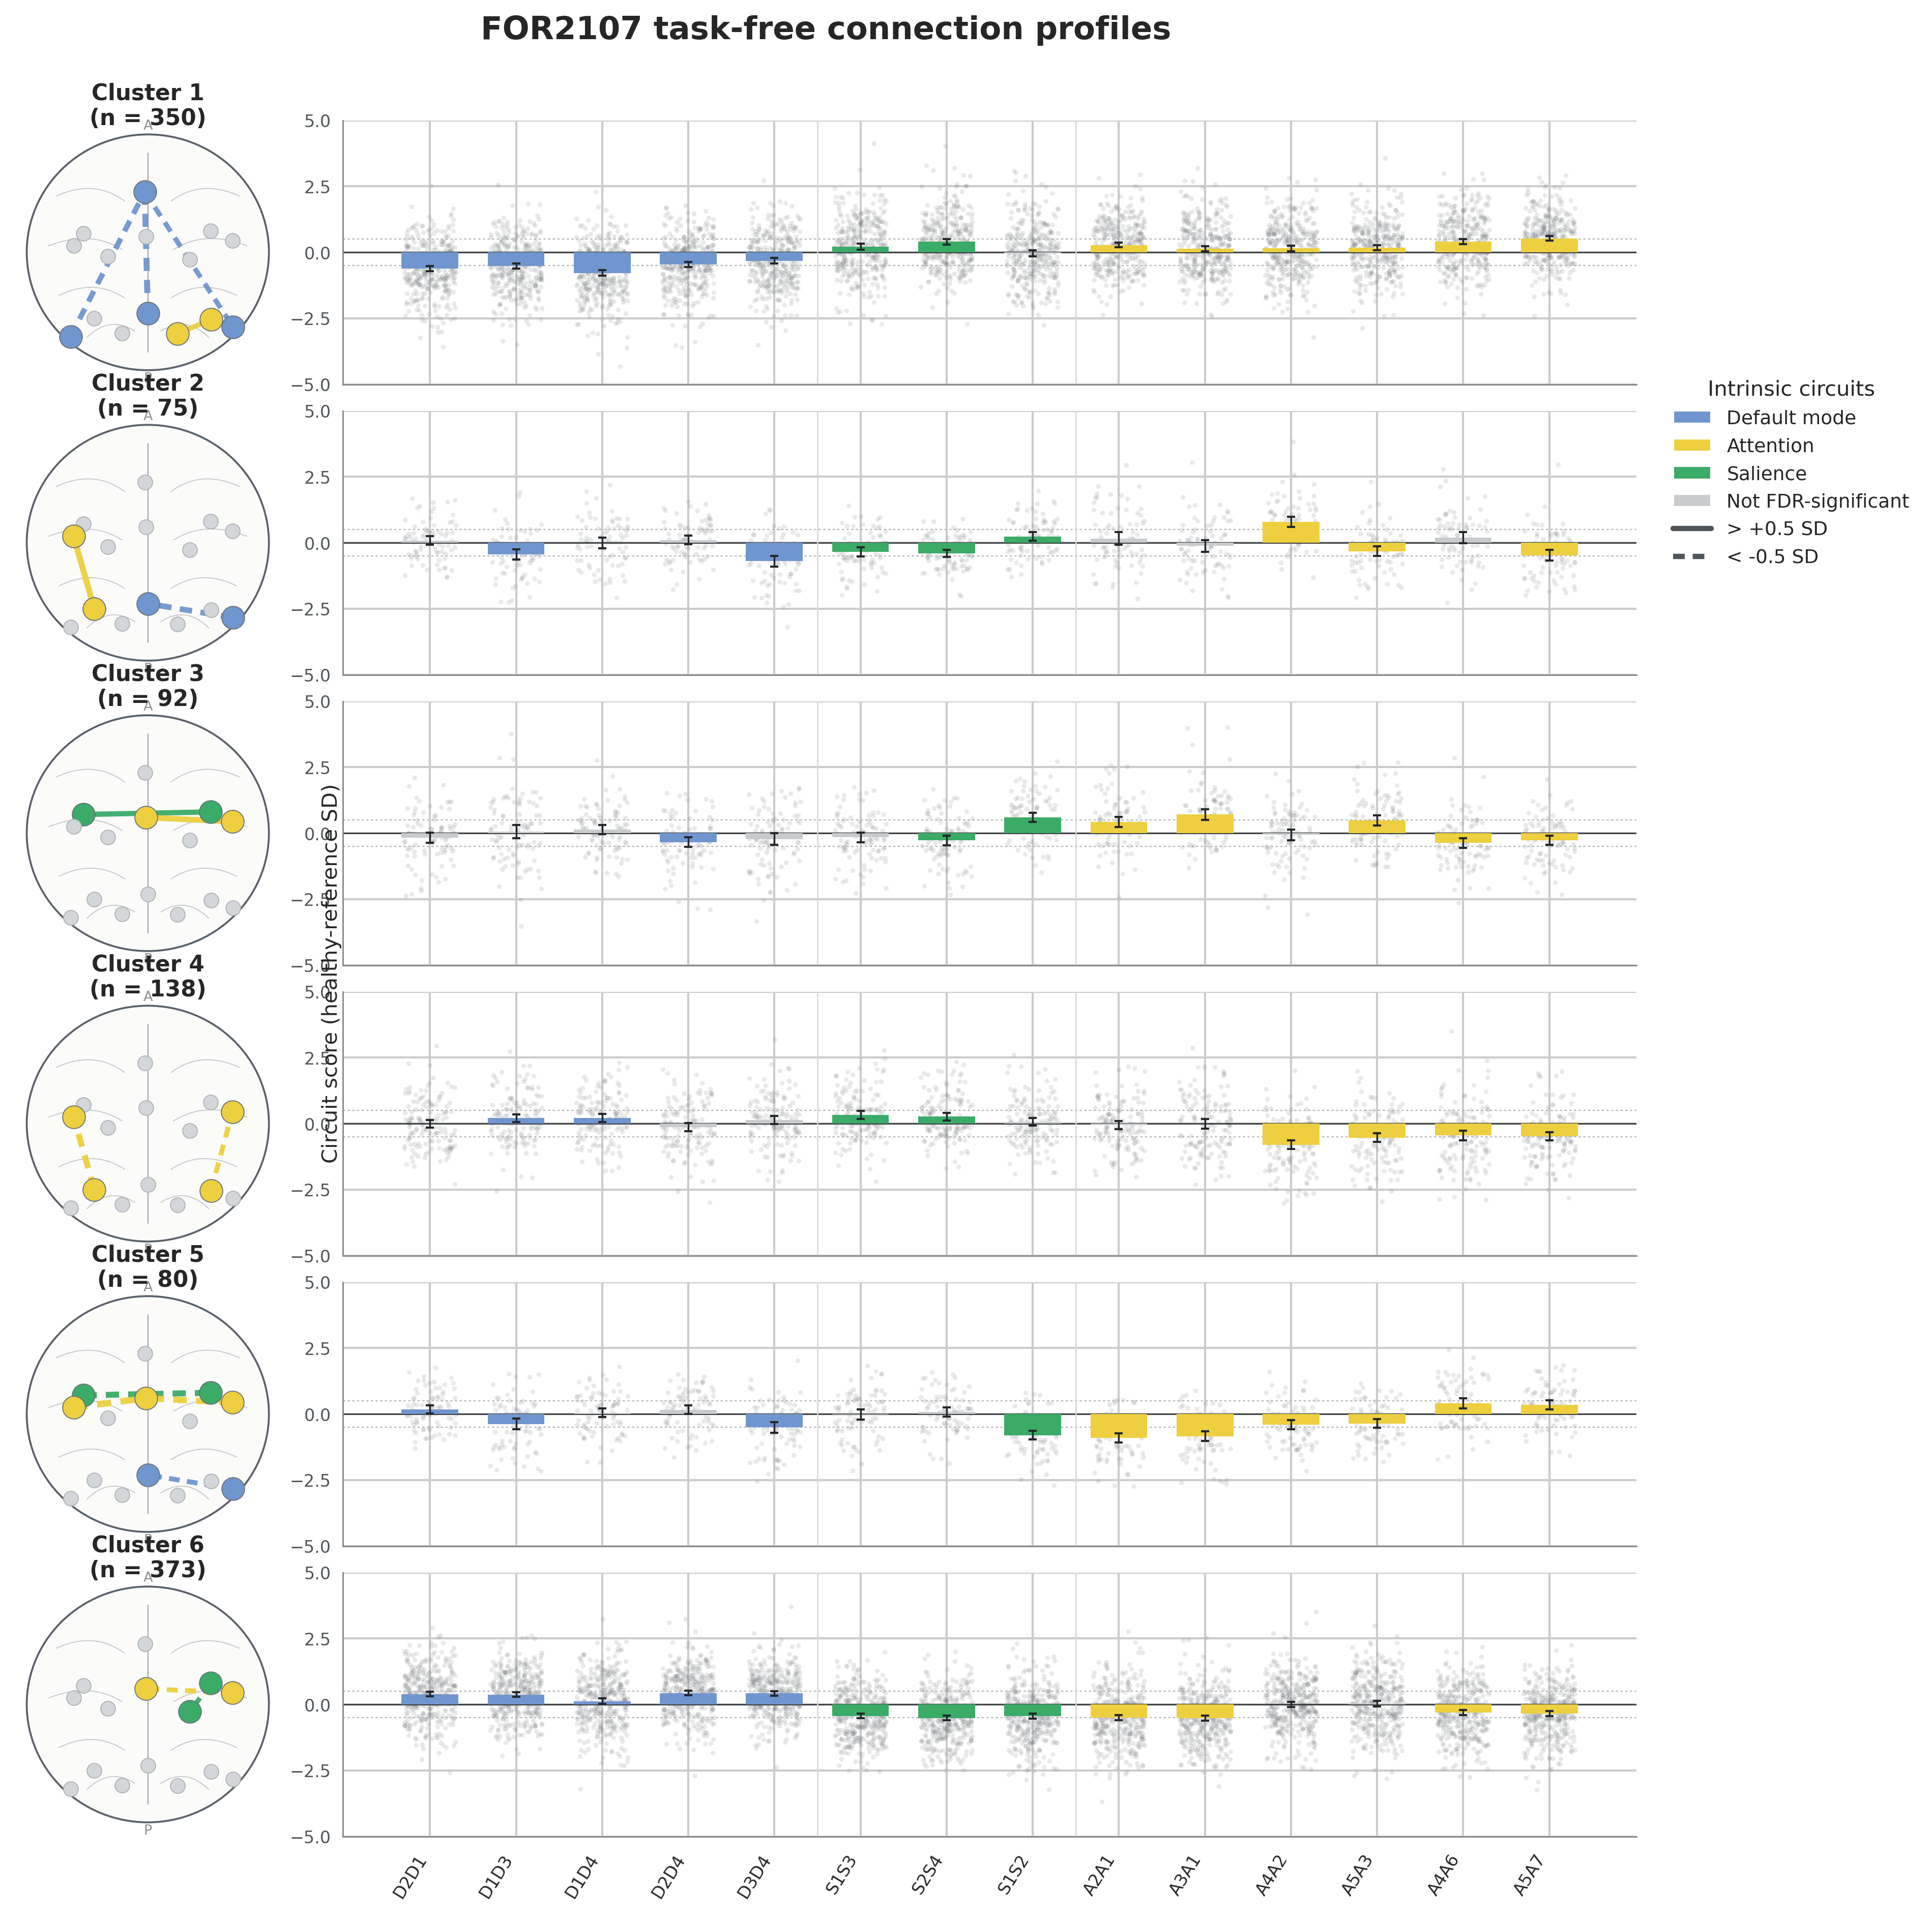
\includegraphics[width=\linewidth,height=.75\textheight,keepaspectratio]{figures/tozzi_style_k6.png}\par
  \end{column}
  \begin{column}{.325\textwidth}
    \centering\paneltitle{FOR2107 · k = 5}\par\vspace{.06cm}
    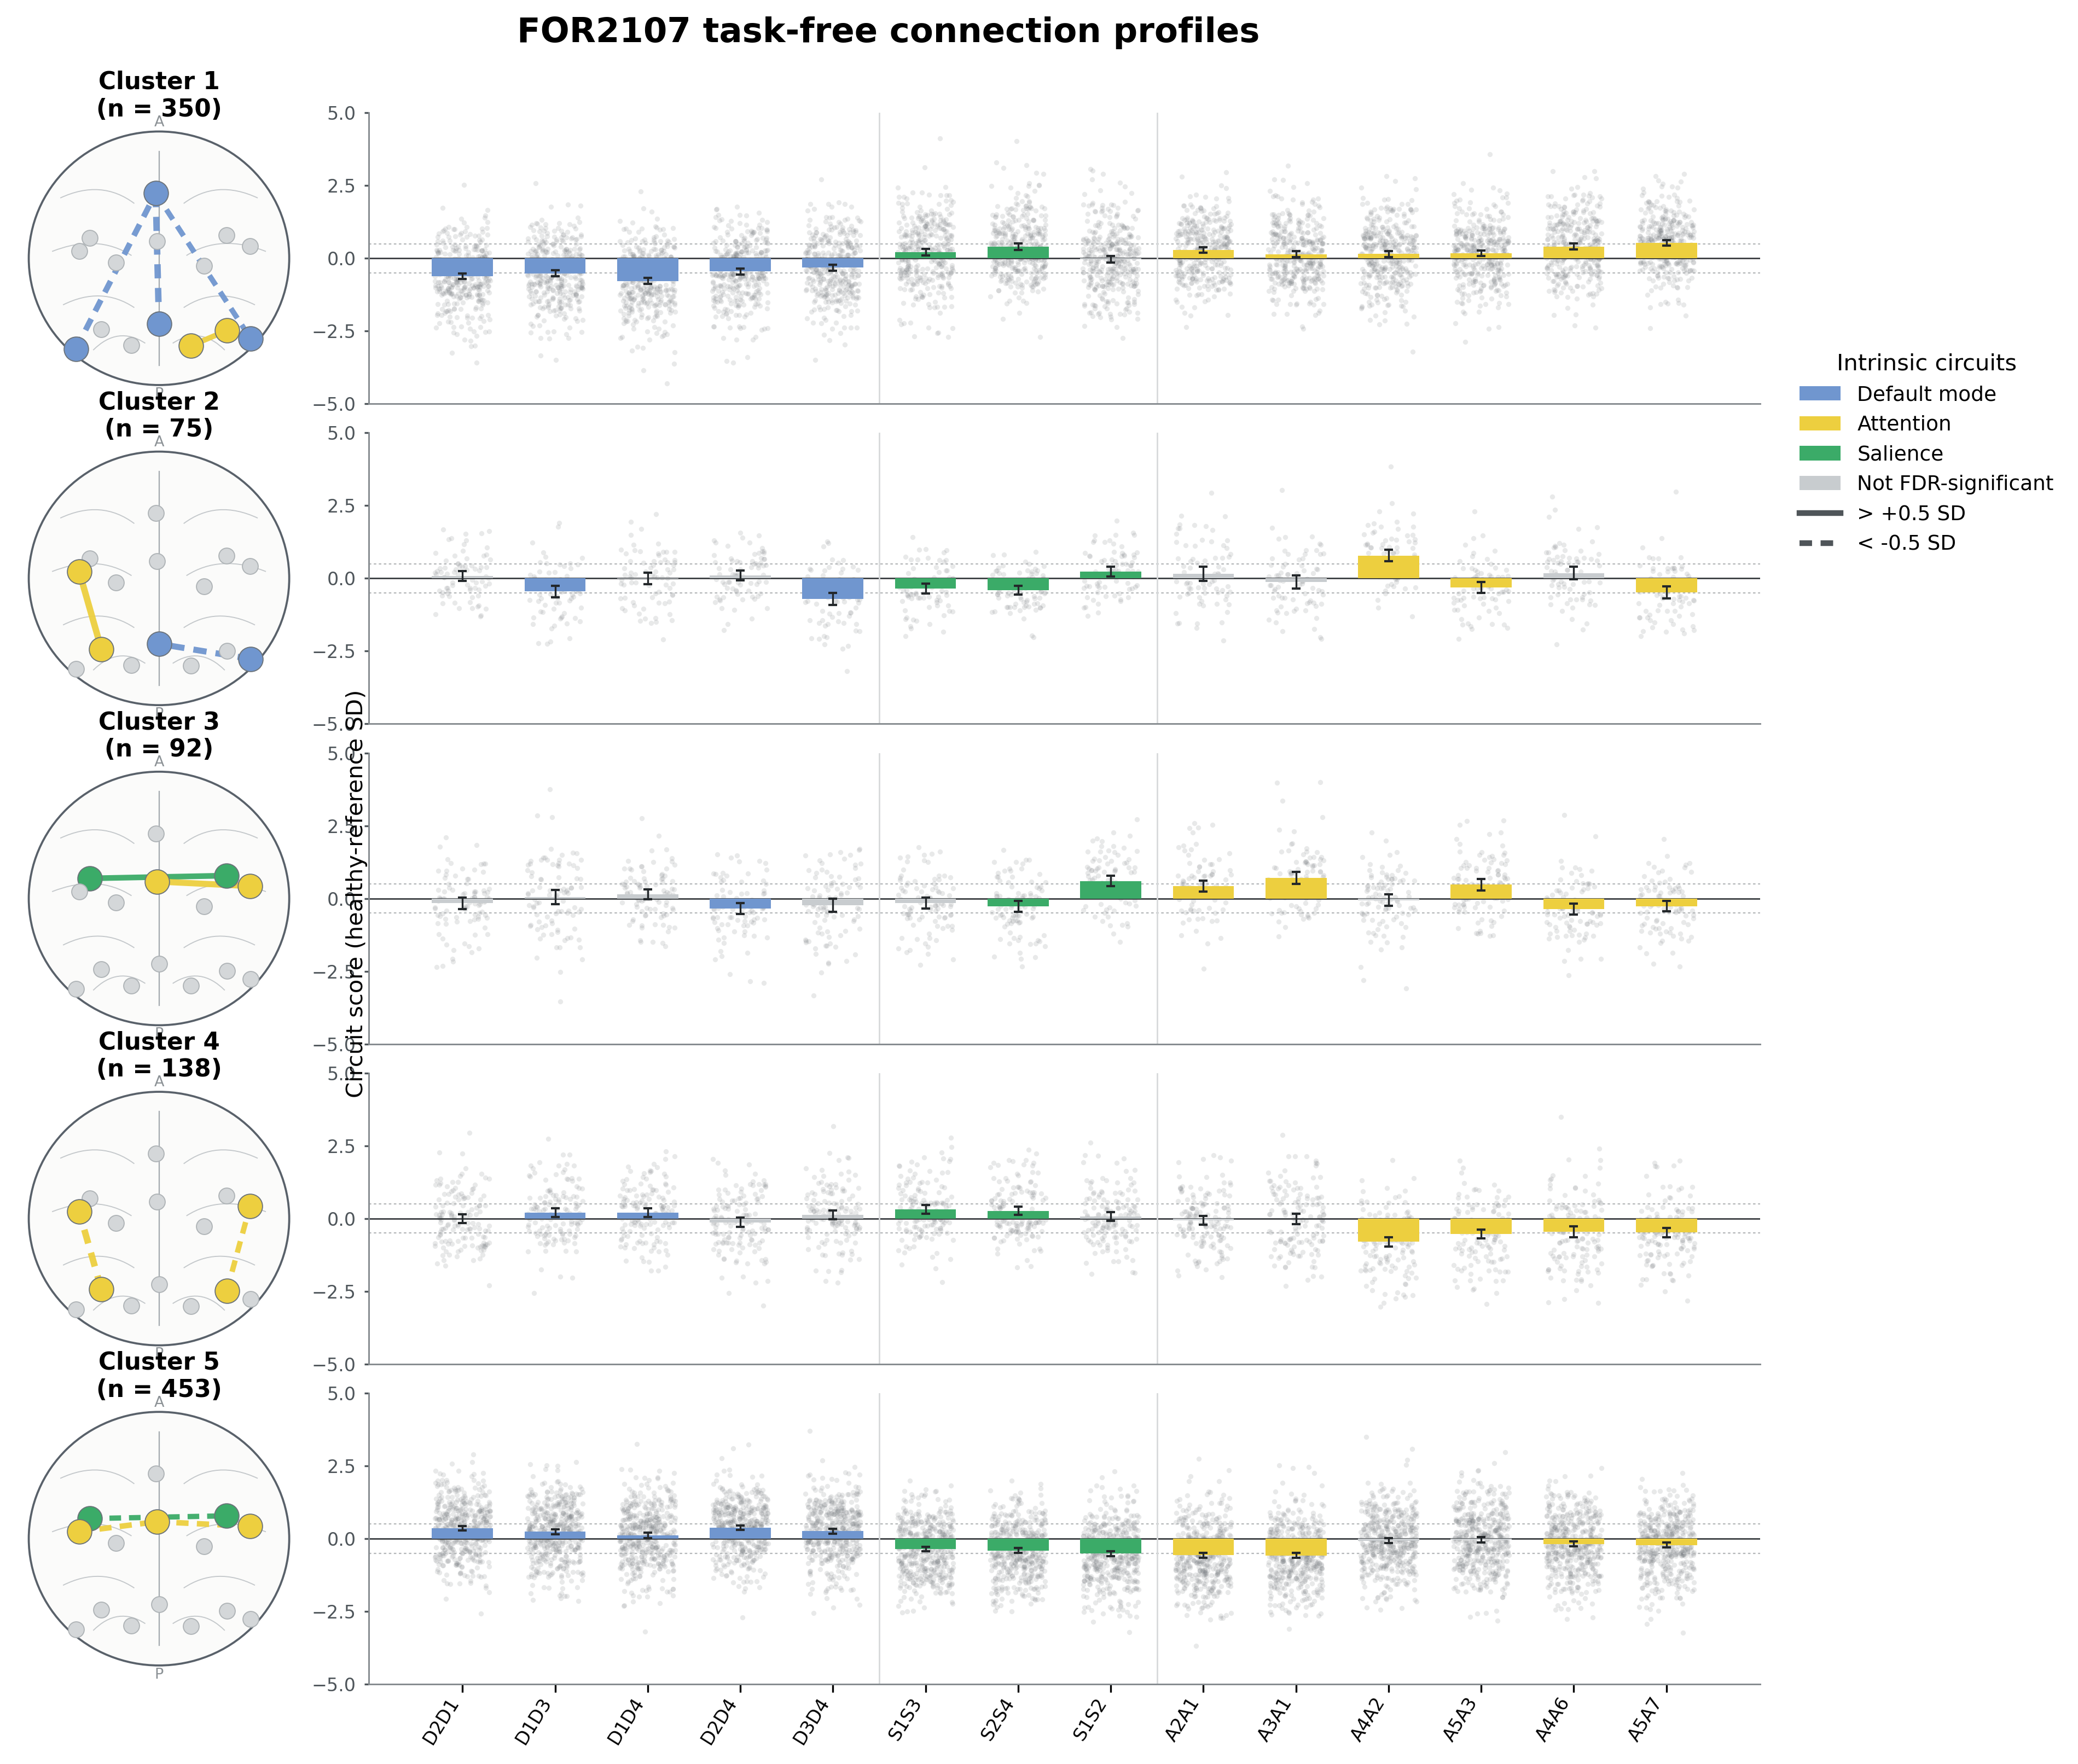
\includegraphics[width=\linewidth,height=.75\textheight,keepaspectratio]{figures/tozzi_style_k5.png}\par
  \end{column}
\end{columns}
\end{frame}

\begin{frame}{Why an exact replication needs Go/NoGo data}
\begin{columns}[T,onlytextwidth]
  \begin{column}{.56\textwidth}
    \begin{beamercolorbox}[rounded=true,sep=.34cm,wd=\linewidth]{normal text}
      {\color{Navy}\fontsize{17}{20}\selectfont\bfseries The missing task removes a defining part of the experiment.}\par\vspace{.18cm}
      {\color{Ink}\normalsize Tozzi’s biotypes were built from a combined profile of resting-state connectivity, task connectivity, and task activation.}\par\vspace{.14cm}
      {\color{Muted}\small The Go/NoGo task supplied the cognitive-control features that distinguished several of the reported six profiles.}
    \end{beamercolorbox}
  \end{column}
  \begin{column}{.40\textwidth}
    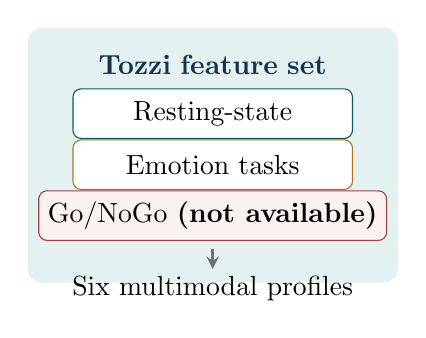
\begin{tikzpicture}[x=1cm,y=.78cm]
      \fill[Teal!12,rounded corners=5pt] (0,0) rectangle (4.7,4.15);
      \node[align=center,text width=4.1cm] at (2.35,3.55) {\color{Navy}\bfseries Tozzi feature set};
      \node[draw=Teal!65!black,fill=white,rounded corners=3pt,minimum width=3.55cm,minimum height=.63cm,align=center] at (2.35,2.75) {Resting-state};
      \node[draw=Amber!80!black,fill=white,rounded corners=3pt,minimum width=3.55cm,minimum height=.63cm,align=center] at (2.35,1.92) {Emotion tasks};
      \node[draw=Red!80!black,fill=Red!8,rounded corners=3pt,minimum width=3.55cm,minimum height=.63cm,align=center] at (2.35,1.09) {Go/NoGo \textbf{(not available)}};
      \draw[-stealth,line width=1pt,color=Muted] (2.35,.55)--(2.35,.22);
      \node[align=center,text width=4cm] at (2.35,-.10) {Six multimodal profiles};
    \end{tikzpicture}
  \end{column}
\end{columns}
\vspace{-.14cm}
\begin{beamercolorbox}[rounded=true,sep=.15cm,wd=.96\textwidth]{normal text}
\centering\color{Red}\normalsize\bfseries Without Go/NoGo: no exact Tozzi replication.\par
\color{Navy}\small We can test a resting-plus-emotion adaptation, but its cluster count and biotype labels would be a new scientific result—not a replication.
\end{beamercolorbox}
\end{frame}

\end{document}
